\chapter{METODOLOGÍA}
\thispagestyle{empty}

\begin{itemize}[leftmargin=1em]
    \item La siguiente Tabla \ref{tab:my-table1} es de clasificación de suelos:
\end{itemize}
\begin{table}[H]
\centering
\begin{threeparttable}
\caption[Clasificación de suelos]{Clasificación de suelos para determinarlo en el laboratorio del departamento de ordenamiento territorial}
\label{tab:my-table1}
\begin{tabular}{@{}ccccc@{}}
\hline
\multicolumn{1}{|c|}{} &
  \multicolumn{1}{c|}{BRITÁNICO} &
  \multicolumn{1}{c|}{AASHTO} &
  \multicolumn{1}{c|}{ASTM} &
  \multicolumn{1}{c|}{SUCS} \\ \cline{2-5} 
\multicolumn{1}{|c|}{\multirow{-2}{*}{SISTEMAS}} &
  \multicolumn{1}{c|}{{\color[HTML]{4D5156} (mm)}} &
  \multicolumn{1}{c|}{{\color[HTML]{4D5156} (mm)}} &
  \multicolumn{1}{c|}{{\color[HTML]{4D5156} (mm)}} &
  \multicolumn{1}{c|}{{\color[HTML]{4D5156} (mm)}} \\ \hline
\multicolumn{1}{|c|}{Grava} &
  \multicolumn{1}{c|}{60 - 2} &
  \multicolumn{1}{c|}{75 - 2} &
  \multicolumn{1}{c|}{\textgreater 2} &
  \multicolumn{1}{c|}{75 - 4,75} \\ \hline
\multicolumn{1}{|c|}{Arena} &
  \multicolumn{1}{c|}{2 - 0,006} &
  \multicolumn{1}{c|}{2 - 0,05} &
  \multicolumn{1}{c|}{2 - 0,075} &
  \multicolumn{1}{c|}{4,75 - 0,075} \\ \hline
\multicolumn{1}{|c|}{Limo} &
  \multicolumn{1}{c|}{0,06 - 0,002} &
  \multicolumn{1}{c|}{0,05 - 0,002} &
  \multicolumn{1}{c|}{0,075 - 0,005} &
  \multicolumn{1}{c|}{\textless 0,075 FINOS} \\ \hline
\multicolumn{1}{|c|}{Arcilla} &
  \multicolumn{1}{c|}{\textless  0,002} &
  \multicolumn{1}{c|}{\textless  0,002} &
  \multicolumn{1}{c|}{\textless  0,005} &
  \multicolumn{1}{c|}{} \\ \hline
\end{tabular}
    \begin{tablenotes}
    \vspace{-0.5cm}
      \item {{\fontsize{10pt}{ \baselineskip}\selectfont \textbf{FUENTE}: Elaboración propia}}
    \end{tablenotes}
\end{threeparttable}
\end{table}


\begin{table}[H]
\centering
\begin{threeparttable}
\caption[Estaciones meteorológicas]{\textbf{Estaciones meteorológicas}}
\label{tab:my-table}
\begin{tabular}{@{}lcccc@{}}
\hline
Estaciones & Este (m) & Norte (m) & Latitud & Longitud \\ \hline
Tunel cero & 490680.81 & 8534186.15 & 13$^{\circ}$15'33.54'' & 75$^{\circ}$5'8'' \\
Ocucaje & 426464.86 & 8410316.41 & 14$^{\circ}$22'42.2'' & 75$^{\circ}$40'0'' \\ \hline
\end{tabular}
    \begin{tablenotes}
    \vspace{-0.5cm}
      \item {{\fontsize{10pt}{ \baselineskip}\selectfont \textbf{FUENTE}: Elaboración propia}}
    \end{tablenotes}
\end{threeparttable}
\end{table}

\begin{table}[H]
\centering
  \begin{threeparttable}
\caption{Estaciones meteorológicas}
\label{tab:my-table2}
\begin{tabular}{@{}lcccc@{}}
\hline
Estaciones & Este (m) & Norte (m) & Latitud & Longitud \\ \hline
Tunel cero & 490680.81 & 8534186.15 & 13$^{\circ}$15'33.54'' & 75$^{\circ}$5'8'' \\
Ocucaje & 426464.86 & 8410316.41 & 14$^{\circ}$22'42.2'' & 75$^{\circ}$40'0'' \\ \hline
\end{tabular}
    \begin{tablenotes}
    \vspace{-0.5cm}
      \item {{\fontsize{10pt}{ \baselineskip}\selectfont \textbf{FUENTE}: Elaboración propia}}
    \end{tablenotes}
\end{threeparttable}
\end{table}

\begin{figure}[H]
    \centering
      \caption{Comparación entre Qdisponible y Qdemanda}
        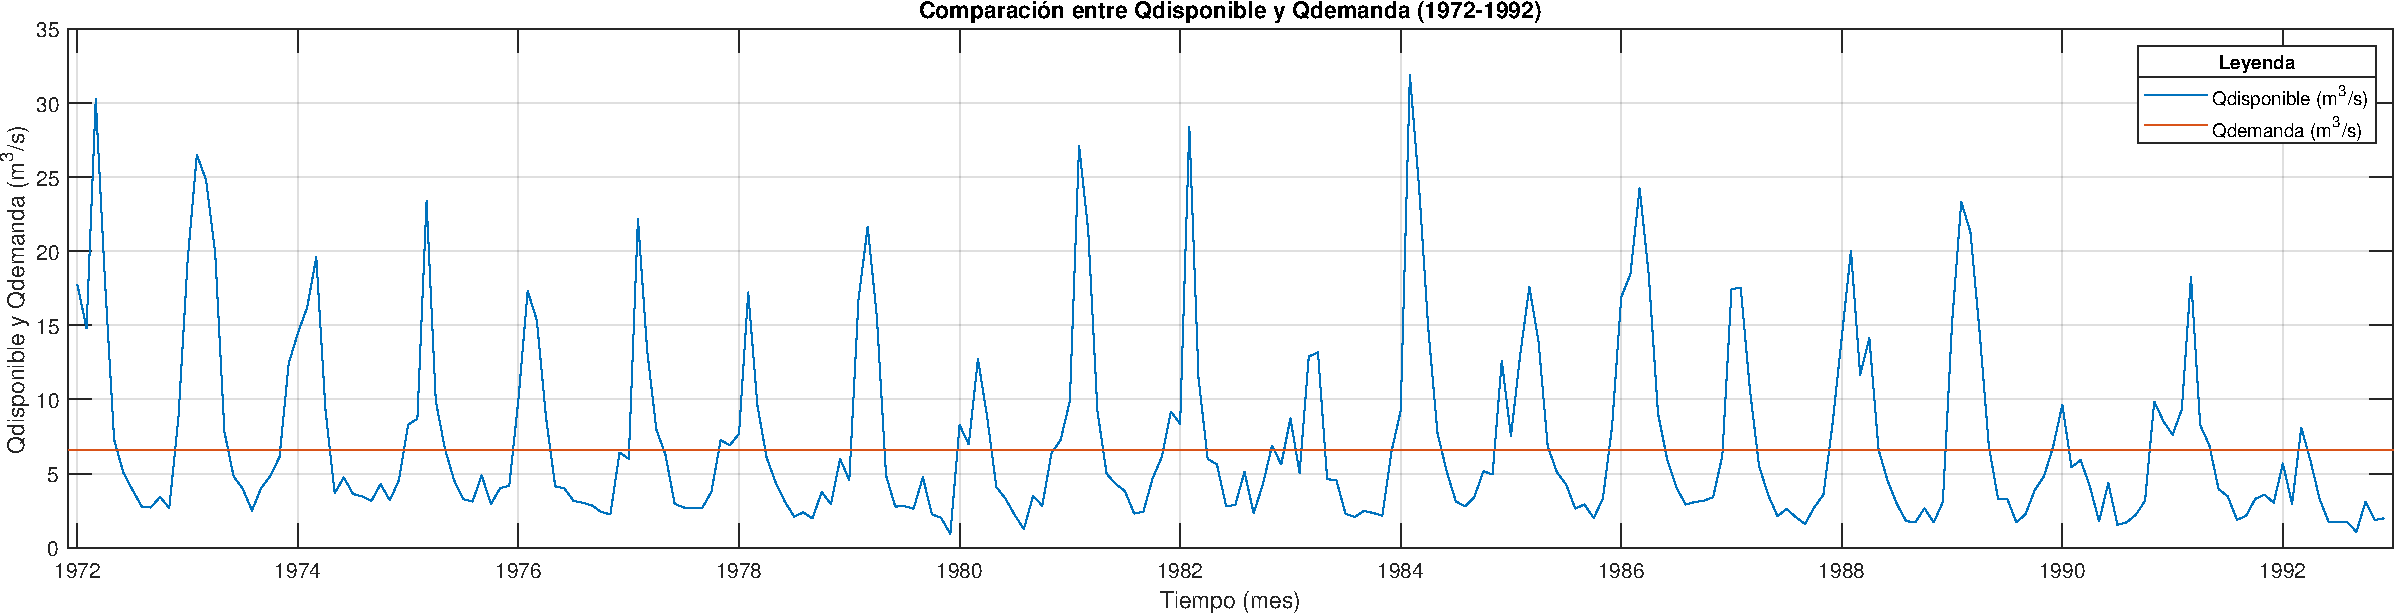
\includegraphics[width=0.7\textwidth]{Figures/Comparation.pdf}
        \captionsetup{labelfont=rm,skip=2pt,textfont=rm,font=small}
        \caption*{\textbf{FUENTE:} Elaboración propia}
    \label{fig:12}
\end{figure}

\begin{itemize}
    \item En la Figura \ref{fig:21}, se muestran los volúmenes medios mensuales acumulados de la estación Santa Eulalia (1972-1992).
\end{itemize}

\begin{figure}[H]
    \centering
    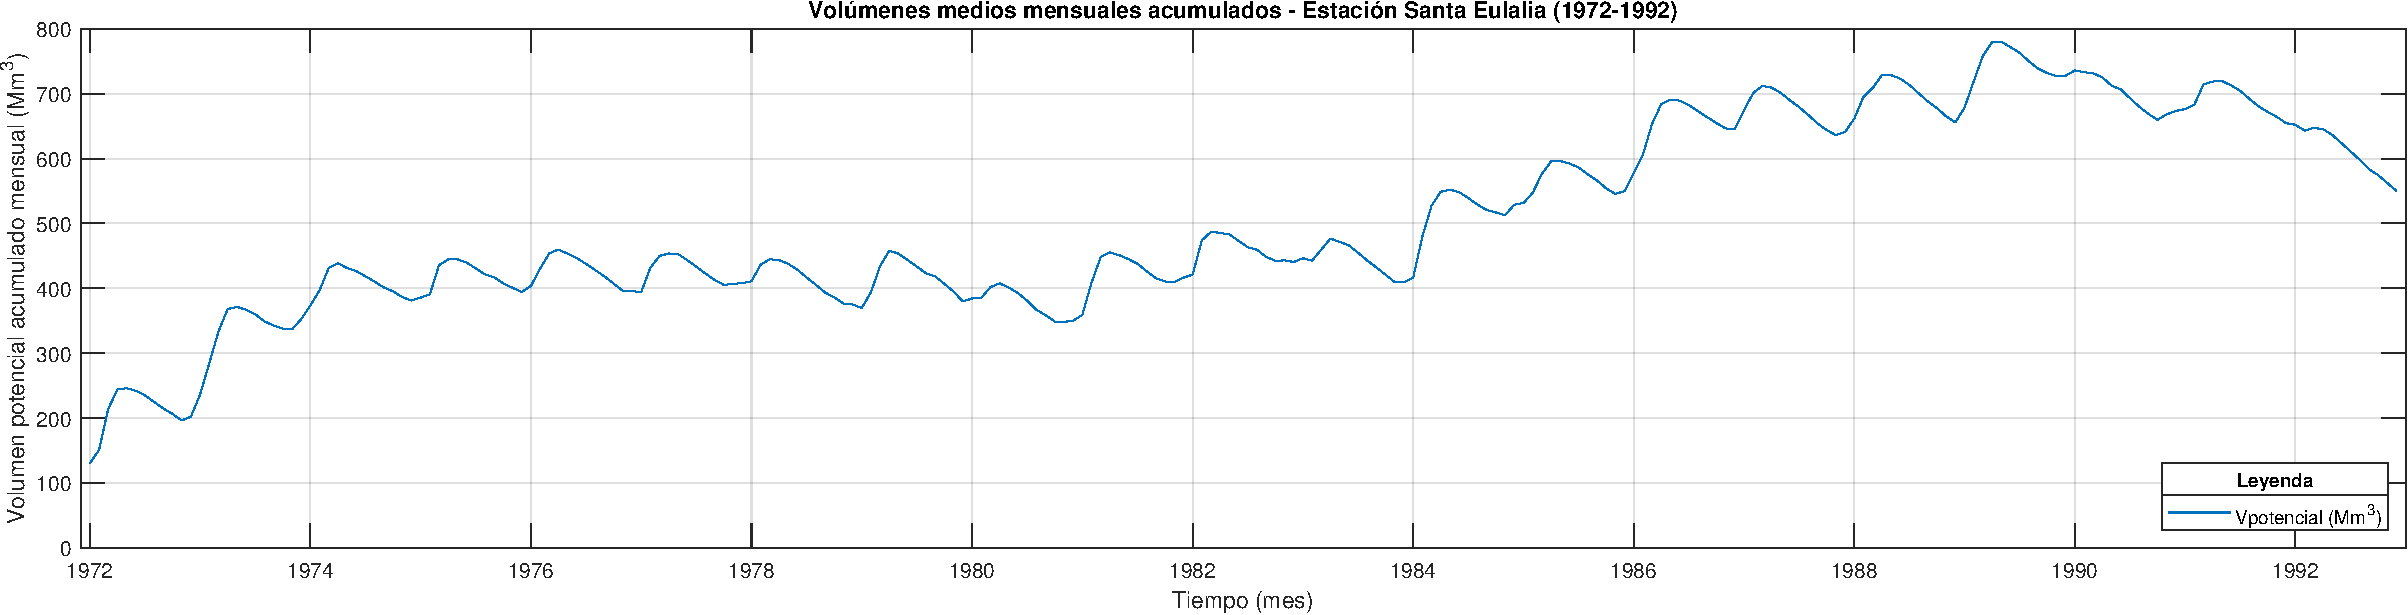
\includegraphics[width=0.7\textwidth]{Figures/Volumenes.pdf}
    \caption{Volúmenes medios mensuales acumulados}
    \captionsetup{labelfont=rm,skip=2pt,textfont=rm,font=small}
        \caption*{\textbf{FUENTE:} Servicio Nacional de Meteorología e Hidrología del Perú SENAMHI}
    \label{fig:21}
\end{figure}

\begin{table}[H]
\centering
  \begin{threeparttable}
    \caption{Sample ANOVA table}
     \begin{tabular}{lllll}
        \toprule \toprule
        Stubhead & \( df \) & \( f \) & \( \eta \) & \( p \) \\
        \midrule
                 &     \multicolumn{4}{c}{Spanning text}     \\
        Row 1    & 1        & 0.67    & 0.55       & 0.41    \\
        Row 2    & 2        & 0.02    & 0.01       & 0.39    \\
        Row 3    & 3        & 0.15    & 0.33       & 0.34    \\
        Row 4    & 4        & 1.00    & 0.76       & 0.54    \\
        \bottomrule
     \end{tabular}
    \begin{tablenotes}
    \vspace{-0.5cm}
        \item {{\fontsize{10pt}{ \baselineskip}\selectfont \textbf{FUENTE}: Elaboración propia}}
    \end{tablenotes}
\end{threeparttable}
\end{table}




